\documentclass[11pt]{article}
\usepackage{graphicx}
\usepackage{cite}
\usepackage{geometry}
\geometry{a4paper}
\usepackage{float}
\begin{document}

\title{Filament Model}
\author{Simon Freedman}
\date{}
\maketitle
\section{Model} 
Actin networks are modeled as collections of actin filaments.
Actin filaments are composed of cylindrical rods and links.  
In general, I'll try to keep the notation that when something is bolded, it has $x$ and $y$ components. 
\subsection{Rods}
\begin{enumerate}
  \item length $l_{rod}$ $\left[units: \mu m\right]$
  \item diameter $d$ $\left[\mu m\right]$
  \item $\mathbf{r^{rod}} = (x^{rod}_{cm},y^{rod}_{cm})$ Center of mass position of rod $\left[\mu m\right]$
  \item orientation $\theta$ $\left[rad\right]$
  \item viscosity $\nu$ $\left[{\mu m}^2\over s\right]$ viscosity of the fluid in which the rod is immersed
  \item Force triplet $\left\{F^{rod}_{||}, F^{rod}_{\perp}, F^{rod}_{\omega}\right\}$ $[{pN, pN, pN}]$, a triplet of forces that are used
    to update the position, and are themse lves updated throughout the simulation. ($F^{rod}_{\omega}$ is the torque.) 
  \item friction triplet $\left\{f_{||} = {2\pi \nu l_{rod} \over \ln{(l_{rod}/d)}  }, f_{\perp} = 2f_{||},
    f_{\omega} = f_{||}l_{rod}^2/4\right\}$ 
\end{enumerate}
The friction triplet has a source that Shila pointed me too, based on the fact that the rod is cylindrical, but I can't
find it right now
\subsection{Links}
\begin{enumerate}
  \item stretching stiffness $\left[pN/\mu m\right]$
  \item bending stiffness $\left[pN/rad\right]$
  \item link length $l_{link}$ $\left[\mu m\right]$
  \item rod indexes : Links are placed between two rods - indices correspond to which rods in the network ``belong'' to
    the link. In cases where a link is only connected to one rod (i.e., at filament ends) the second rod index is $-1$
  \item  $\mathbf{r^{link}}=(x^{link}_{cm},y^{link}_{cm})$ -- the midpoint between the two rods it
    connects
  \item $\theta^{link}$ (orientation) -- the average angle of the two rods it connects
\end{enumerate}
A number of rods $n_{rod}$ are connected with links make up a filament. Links are placed at the ends of filaments so
that the total number of links per filament is $n_{rod} + 1$. A number of filaments $n_ {fil}$ compose the actin network.
\section{Dynamics} 
\subsection{Calculate bending force}
Bending forces are calculated using a continuum model \cite{nedelec} in which the bending energy is approximated as a
triplet of forces at three contiguous link positions
\begin{eqnarray}
  \mathbf{F}^{link}_{i-1} &=& -\phi\nonumber\\
  \mathbf{F}^{link}_{i} &=& 2\phi\nonumber\\
  \mathbf{F}^{link}_{i+1} &=& -\phi\nonumber\\
  \phi &=& \alpha(\mathbf{r}^{link}_{i-1} - 2\mathbf{r}^{link}_i + \mathbf{r}^{link}_{i+1})\nonumber\\
  \alpha &=& \kappa_B\left( 1\over l_{rod} \right)^3
  \label{eqn:flink}
\end{eqnarray}
where $i$ runs over the rod indices $1\cdots n_{rod}$ and $\kappa_B$ is the bending modulus of the filament, set here to
$10\mu m*kT$, corresponding to the persistence length of actin $~10\mu m$. The force on an individual rod is then
calculated as the average of the forces on the two links at either end. I.e.,
\begin{equation} 
  F^{rod}_i = \left( 1\over2 \right)(\mathbf{F}^{link}_{i-1} + \mathbf{F}^{link}_{i})
  \label{eqn:frod}
\end{equation}
This force vector is then projected onto the rod in terms of ${F^{rod}_{||,i}, F^{rod}_{\perp,i}}$. 
The torque on a rod is calculated using these forces, and the length of the rod. I.e,
\begin{equation}
  F^{rod}_{\omega,i} = \left(  \mathbf{r}^{rod}_{i} - \mathbf{r}^{link}_{i-1}\right)\times F^{link}_{i-1} + 
  \left(  \mathbf{r}^{rod}_{i} - \mathbf{r}^{link}_{i}\right)\times F^{link}_{i}
  \label{eqn:trqrod}
\end{equation}
The force triplet of the rod is updated by adding to it ${F^{rod}_{||,i}, F^{rod}_{\perp,i}, F^{rod}_{\omega,i}}$ from
bending.
\subsection{Calculate stretching force}
Stretching forces are calculated as being proportional to the extension of links, or the end to end distance of a link. 
Since each link is connected to $2$ rods, this amounts to measuring the minimum distance between those two rods. We
label the head of the first rod $\mathbf{h}_{i}$ and the tail of the second rod $\mathbf{t}_{i+1}$, such that $|\mathbf{t}_{i+1} -
\mathbf{h}_i|$ is the minimum distance between the two rods. We then calculate the Hookean spring force as 
\begin{equation}
  \phi = k_s \left( |\mathbf{t}_{i+1}-\mathbf{h}_i|-l_{link} \right)
  \label{eqn:stretch}
\end{equation}
Balancing this force over both rods yields
\begin{eqnarray}
  F_{x,i} &=& \phi\cos{(\theta^{link})}\\\nonumber
  F_{y,i} &=& \phi\sin{(\theta^{link})}\\\nonumber
  F_{x,i+1} &=& -\phi\cos{(\theta^{link})}\\\nonumber
  F_{y,i+1} &=& -\phi\sin{(\theta^{link})}\\\nonumber
  \label{eqn:stretch_comp}
\end{eqnarray}
These values are used to calculate the parallel and perpendicular components of the force on the rod. Since this
stretching happens at the end of the rod, the torque at the center of the rod is calculated as
\begin{eqnarray}
  F_{\omega,i} &=& (\mathbf{h}_i-\mathbf{r}^{rod}_i) \times \mathbf{F}_i\\\nonumber
  F_{\omega,i+1} &=& (\mathbf{t}_{i+1}-\mathbf{r}^{rod}_{i+1}) \times \mathbf{F}_{i+1}
  \label{eqn:stretch_trq}
\end{eqnarray}
\subsection{Rod Update}
The equation of motion for rod $i$ is
\begin{eqnarray}
  \mathbf{r}(t+\delta t) &=& \mathbf{r}(t) + \mathbf{v} \delta t\\\nonumber
  \mathbf{v}_{j} &=& {F_{j}\over f_{j}} + \sqrt{{4kT\over \delta t*f_j}rng_{0,1}} 
  \label{eqn:motion}
\end{eqnarray}
where $j$ runs over the three components of F and f, $\left\{ ||, \perp, \omega\right\}$, and $rng_{0,1}$ represents a
random number i n the range $\left[ 0,1 \right]$ taken from a normal distribution, representing the Brownian component. 
(Note: this equation was already in Shila's simulation-- I have to ask him for the source.) 
The force triplet of the rod is updated by adding to it the calculated ${F^{rod}_{||,i}, F^{rod}_{\perp,i},
F^{rod}_{\omega,i}}$ from stretching.
\section{Persistence Length Calculation}
The persistence length $L_p$ has been calculated experimentally by plotting the correlation of tangent vectors along a
filament as a function of distance \cite{ott}
\begin{equation}
  <\mathbf{t}(s)\cdot\mathbf{t}(s+x)>=exp(-x/2L_p)
  \label{eqn:pl}
\end{equation}
where $x$ is the distance from the initial position $s$ along the filament and $\mathbf{t}(s)$ is the tangent vector at $s$.
In simulation, this calculation becomes 
\begin{equation}
  {1\over N_t}\sum_{t=t_{relaxed}}^{t_{final}}{cos(\theta^{rod}_i -
  \theta^{rod}_0)}=exp(-|\mathbf{r}^{rod}_i-\mathbf{r}^{rod}_0|/2L_p)
  \label{eqn:pl_discrete}
\end{equation}
where $N_t$ is the number of timesteps, $t_{relax}$ is usually about half the total simulation, and $t_{final}$ is the
end of the simulation. The total number of data points to plot is therefore the number of rods in the filament. 
Figure \ref{fig:pl} shows an example of the results of this measurement, for persistence length calculations at various
viscosities. In each of the plots in figure \ref{fig:pl}, $L_p$ was calculated from a linear fit to the plot and ranged 
from $1.76 - 1.80 \mu m$ with an $R^2$ mean error of $~0.81$. These plots look more like an exponential decay then a
linear one, so it would seem like there's something wrong with this model.  
\begin{figure}[H]
  \centering
  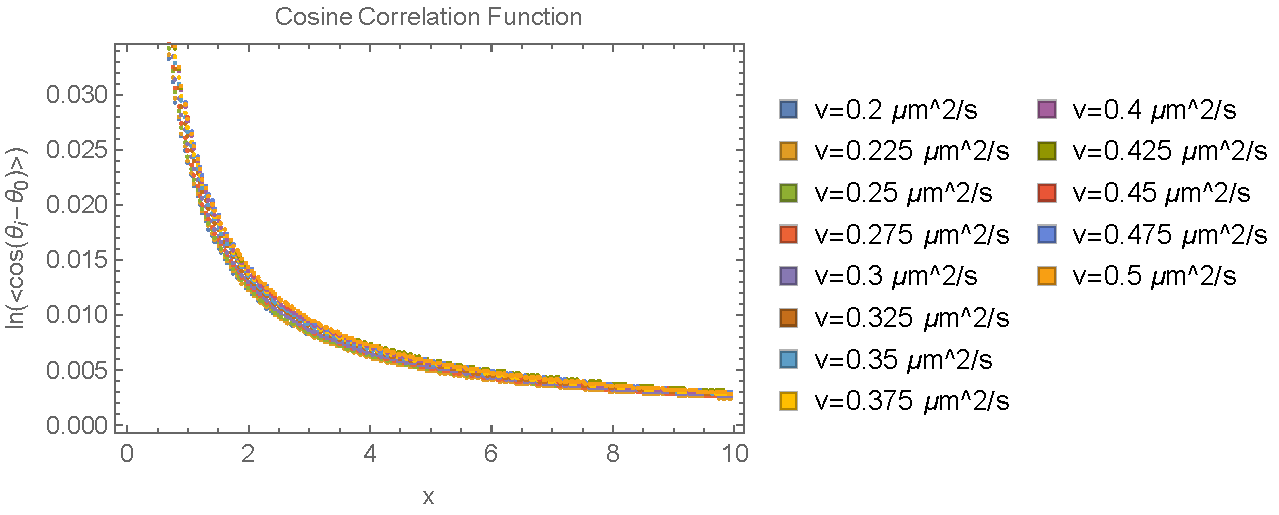
\includegraphics[width=0.75\textwidth]{pl-calc-ccf.pdf}
\caption{Persistence length calculations at various viscosities, $v$. Here we set $n_{rod} = 200$, $l_{rod}=0.05 \mu m$, 
$l_{link} = l_{rod}/10$, $k_s = 200 pN/\mu m$, $\kappa_B = 10\mu m*kT$, $kT =
0.004 pN-\mu m$, $dt = 0.0001 s$, and $t_{final} = 100 s$. } 
  \label{fig:pl}
\end{figure}
\section{Time}
The simulations in figure \ref{fig:pl} each took about a half hour to complete (but were run concurrently using Slurm
arrays). For bigger simulations where I have motors $~100$ motors, $~100$ filaments, with $n_{rod}\approx 10$, the whole
simulation will take around $4$ or $5$ hours.
\bibliography{actin_model}
\bibliographystyle{plain}
\end{document}
